
\begin{frame}
	\frametitle{Über \LaTeX}

	\begin{itemize}
		\itemra ein Textsatzsystem
        \itemra \TeX{} ist eine Programmiersprache von Donald E. Knuth
        \itemra \LaTeX{} ist eine Sammlung von Makros für \TeX{} von Leslie Lamport
		\itemra Dokumente werden aus Quelltext erzeugt
		\itemra Quelltext ist ``logisches Markup'' (wie HTML)
		\itemra kein WYSIWYG (\textbf What\textbf You\textbf See\textbf Is\textbf What\textbf You\textbf Get)
		\itemra standardisierte Dokumente
		\itemra einfacher Formelsatz
		\itemra kostenlos und für alle gängigen Betriebssysteme erhältlich
		\itemra Standard für wissenschaftliche Veröffentlichungen
	\end{itemize}
\end{frame}

\begin{frame}
	\frametitle{Woher bekommt man \LaTeX?}
	
	\begin{itemize}
		\item offizielle Homepage: \url{http://www.latex-project.org}
		\item verschiedene Distributionen verfügbar:
		\begin{center}
			\begin{tabular}{rl}
				{\TUgreen TeX Live} & \url{http://tug.org/texlive/} \\
					& Installer oder direkt von USB-Stick startbar\\
				{\TUgreen Mik TeX} & \url{http://www.miktex.org} \\
					& für Windows-Systeme; Installer oder portable Version\\
				{\TUgreen Mac TeX} & \url{http://tug.org/mactex/} \\
					& TeX Live für Apple Mac-Systeme
			\end{tabular}
		\end{center}
		\item detailierte Beschreibung des Installationsvorgangs für \TeX Live:
		\begin{center}
			\url{http://www.dante.de/tex.html}
		\end{center}
	\end{itemize}
\end{frame}

\begin{frame}
	\frametitle{Grundaufbau einer \LaTeX-Datei}
	
	\begin{itemize}
		\item Präambel
			\begin{itemize}
				\item[$\to$] Stilvorgaben (Schriftart, Schriftgröße, Seitenränder, Kopf-/Fußzeile, usw.)
				\item[$\to$] Pakete mit zusätzlichen Funktionen laden (z. B. Farben, Verlinkung, usw.)\\~
			\end{itemize}
		\item Dokument
			\begin{itemize}
				\item[$\to$] Inhaltsverzeichnis
				\item[$\to$] Kapitel und Überschriften
				\item[$\to$] Text und Bilder
				\item[$\Ra$] der gesamte Inhalt
			\end{itemize}
	\end{itemize}
\end{frame}

\begin{frame}[fragile]
	\frametitle{\LaTeX: Ablauf der Dokumenterstellung}

\begin{center}
	\begin{tikzpicture}%[nodes=draw]
	\node[outer sep=5pt, anchor=base]            (a) {~};
	\node[outer sep=5pt, anchor=base] at (5,0) (b) {~};
	\node[outer sep=5pt, anchor=base] at (7,0) (c) {~};
	\node[outer sep=5pt, anchor=base] at (12,0) (d) {~};
	\node[outer sep=5pt, anchor=base] at (14,0) (e) {~};
	\node[outer sep=5pt, anchor=base] at (19,0) (f) {~};
	\path let \p0=($(a.west)-(b.east)$) in
	  (a) --
	  node [
	    pos=.5,
	    auto=false,
	    shape=single arrow,
	    anchor=tail,
	    draw=none,
	%    line join=round,
	    xshift=-veclen(\p0)/2,
	    minimum height=veclen(\p0)-\pgfkeysvalueof{/pgf/outer xsep},
	    fill=TUgreen,
	    decorate, decoration={
	      name=random steps,
	      segment length=+.5pt,
	      amplitude=.5pt}
	  ] {Editor}
	  (b);
\node[align=left] at (2,-2) {zur Eingabe des\\ sog. \textbf{Quellcode}\\(bei uns: Kile)};	  
	  
	\path let \p0=($(c.west)-(d.east)$) in
	  (c) --
	  node [
	    pos=.5,
	    auto=false,
	    shape=single arrow,
	    anchor=tail,
	    draw=none,
	%    line join=round,
	    xshift=-veclen(\p0)/2,
	    minimum height=veclen(\p0)-\pgfkeysvalueof{/pgf/outer xsep},
	    fill=TUgreen,
	    decorate, decoration={
	      name=random steps,
	      segment length=+.5pt,
	      amplitude=.5pt}
	  ] {\LaTeX-Compiler}
	  (d);
\node[align=left] at (9.3,-2) {übersetzt den Quellcode\\ in ein Dokumentformat\\ (z. B. PDF)};	 

	\path let \p0=($(e.west)-(f.east)$) in
	  (e) --
	  node [
	    pos=.5,
	    auto=false,
	    shape=single arrow,
	    anchor=tail,
	    draw=none,
	%    line join=round,
	    xshift=-veclen(\p0)/2,
	    minimum height=veclen(\p0)-\pgfkeysvalueof{/pgf/outer xsep},
	    fill=TUgreen,
	    decorate, decoration={
	      name=random steps,
	      segment length=+.5pt,
	      amplitude=.5pt}
	  ] {Betrachter}
	  (f);
\node[align=left] at (16.6,-2) {zeigt das Dokument an};
	\end{tikzpicture}
\end{center}

\end{frame}



\begin{frame}
	\frametitle{Kile - \LaTeX Entwicklungsumgebung}
	
	\begin{itemize}
			\item erleichtert das Bearbeiten von mehreren Dokumenten
			\item Autovervollständigung
			\item Hilfe zum Kompilieren der Dokumente
			\item Syntaxhervorhebung
			\item Rechtschreibprüfung
			\item Code-Faltung
	\end{itemize}
\end{frame}

\begin{frame}[plain]
	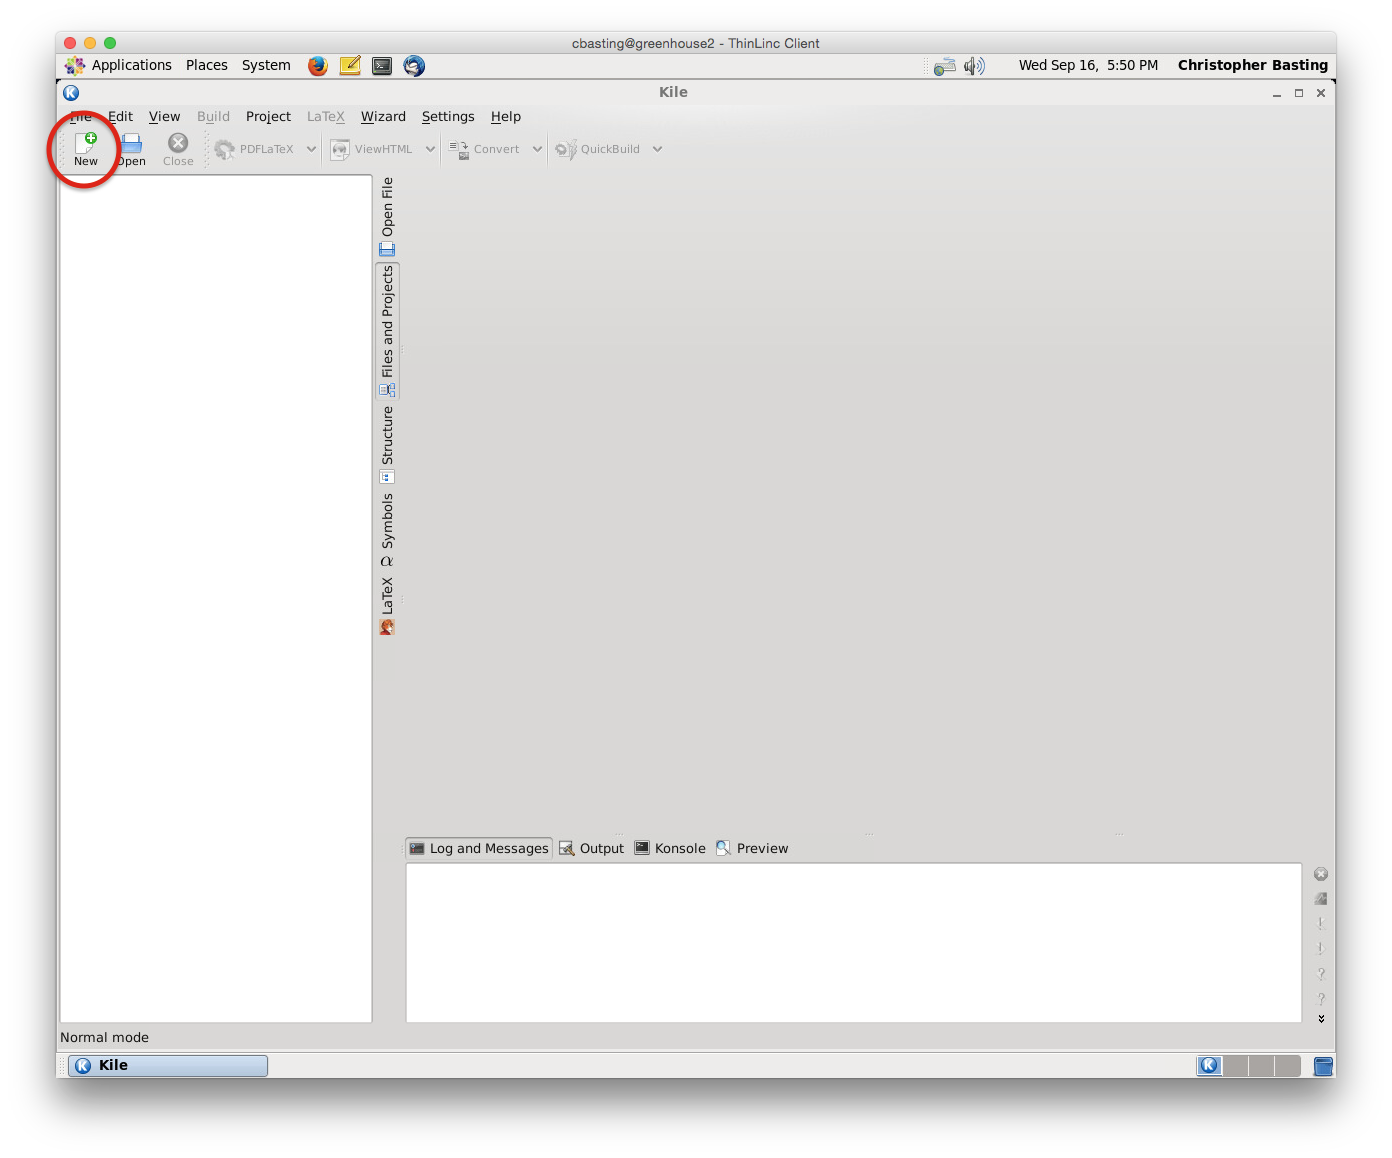
\includegraphics[width=\textwidth]{screenshots/kile-start.png}
\end{frame}

\begin{frame}[plain,noframenumbering]
	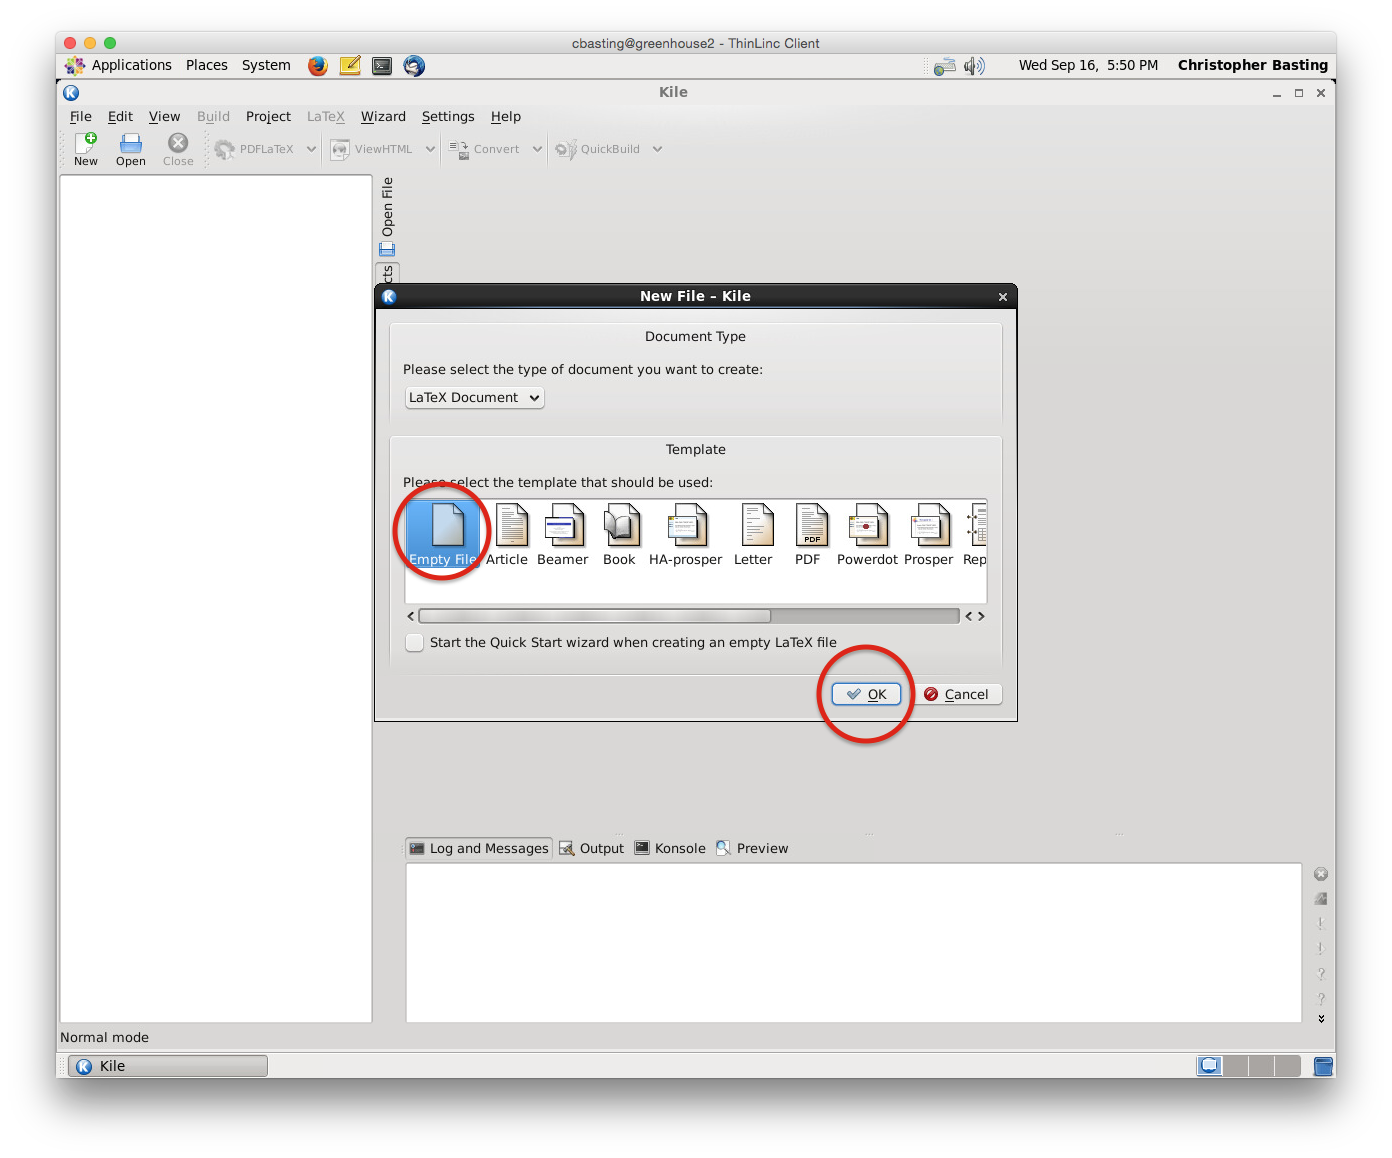
\includegraphics[width=\textwidth]{screenshots/kile-new.png}
\end{frame}

\begin{frame}[plain,noframenumbering]
	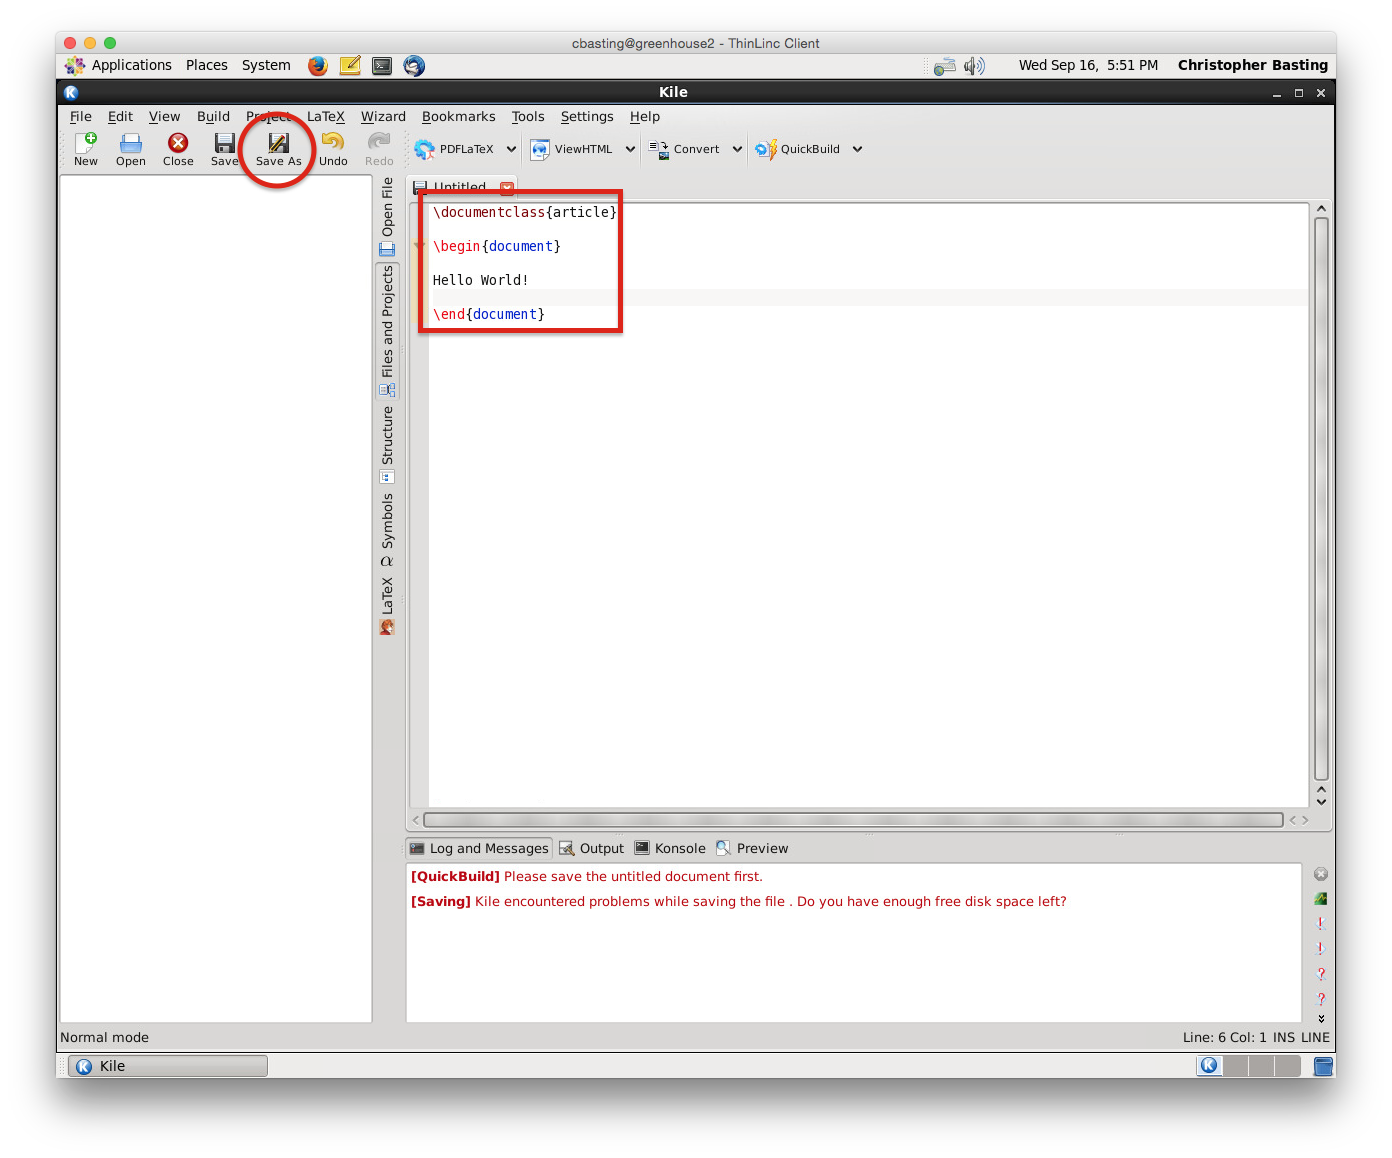
\includegraphics[width=\textwidth]{screenshots/kile-new-doc.png}
\end{frame}

\begin{frame}[plain,noframenumbering]
	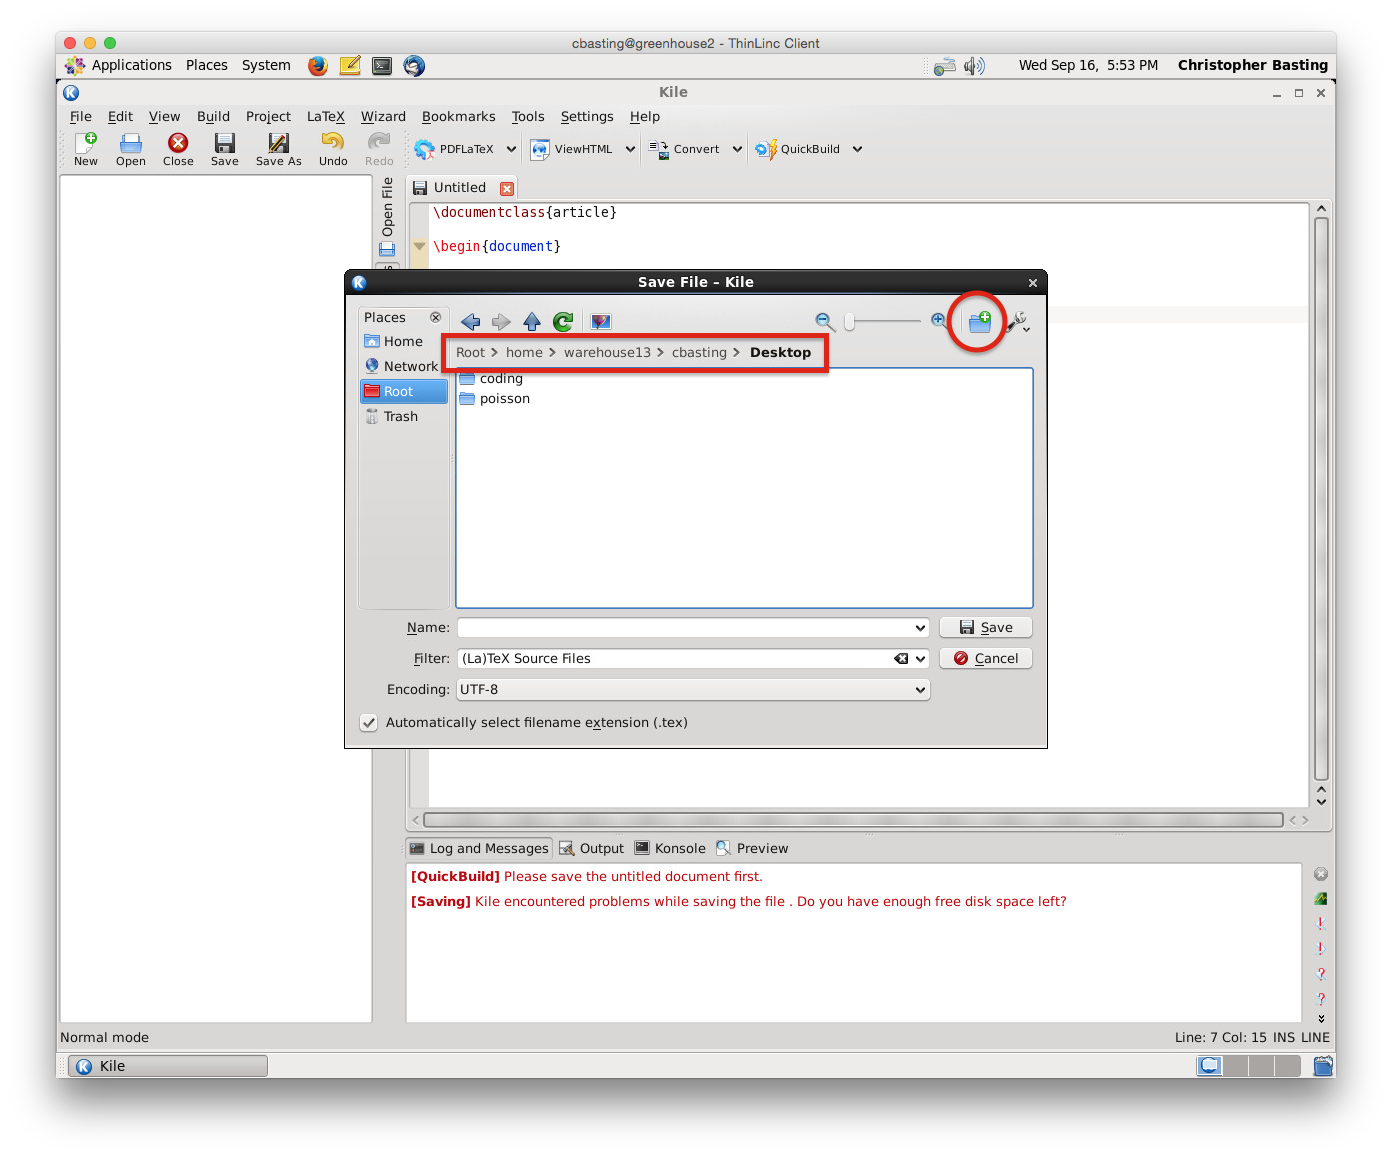
\includegraphics[width=\textwidth]{screenshots/kile-new-save-as.png}
\end{frame}

\begin{frame}[plain,noframenumbering]
	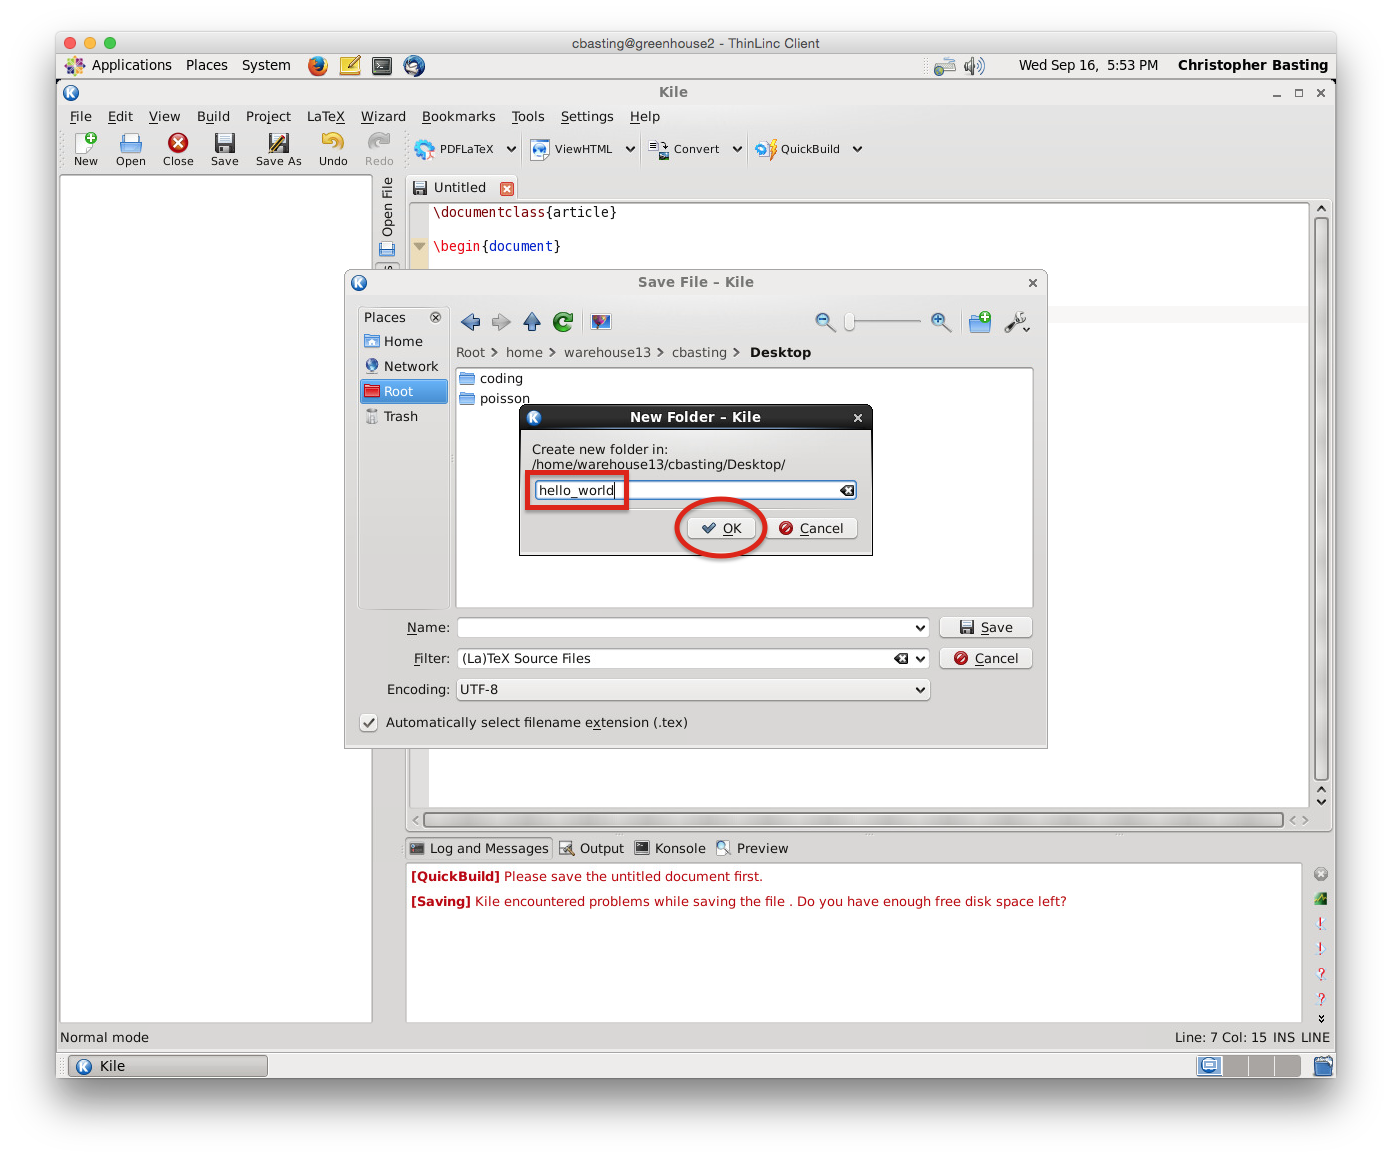
\includegraphics[width=\textwidth]{screenshots/kile-new-save-as-create-folder.png}
\end{frame}

\begin{frame}[plain,noframenumbering]
	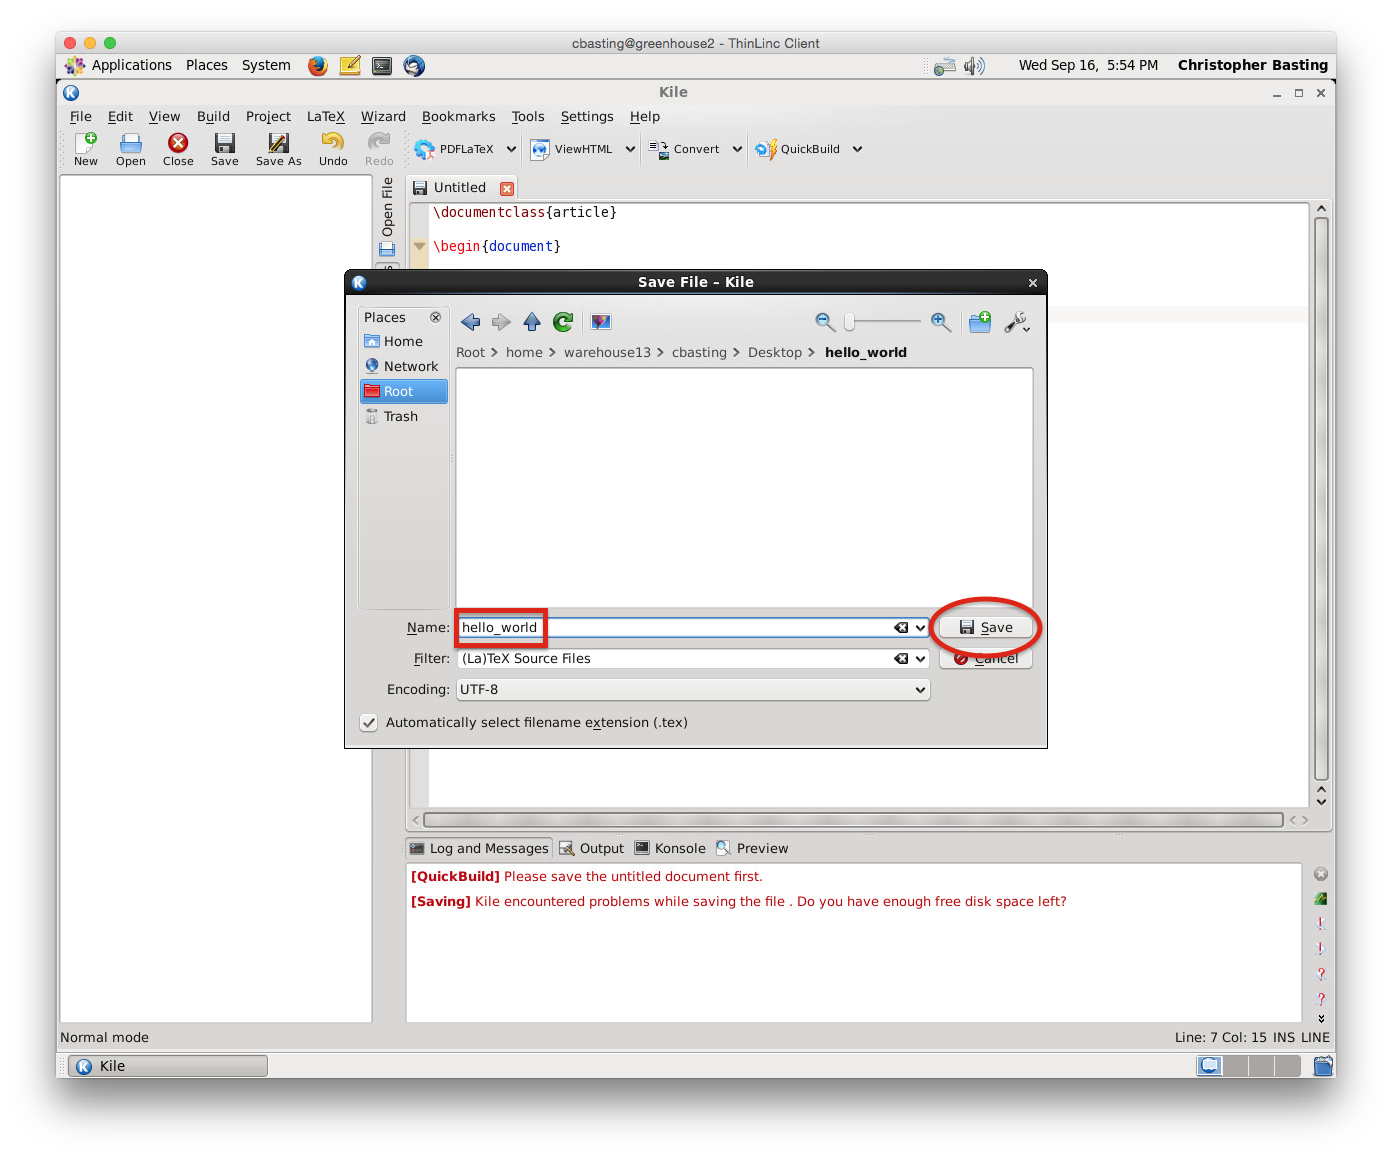
\includegraphics[width=\textwidth]{screenshots/kile-new-save-as-2.png}
\end{frame}

\begin{frame}[plain,noframenumbering]
	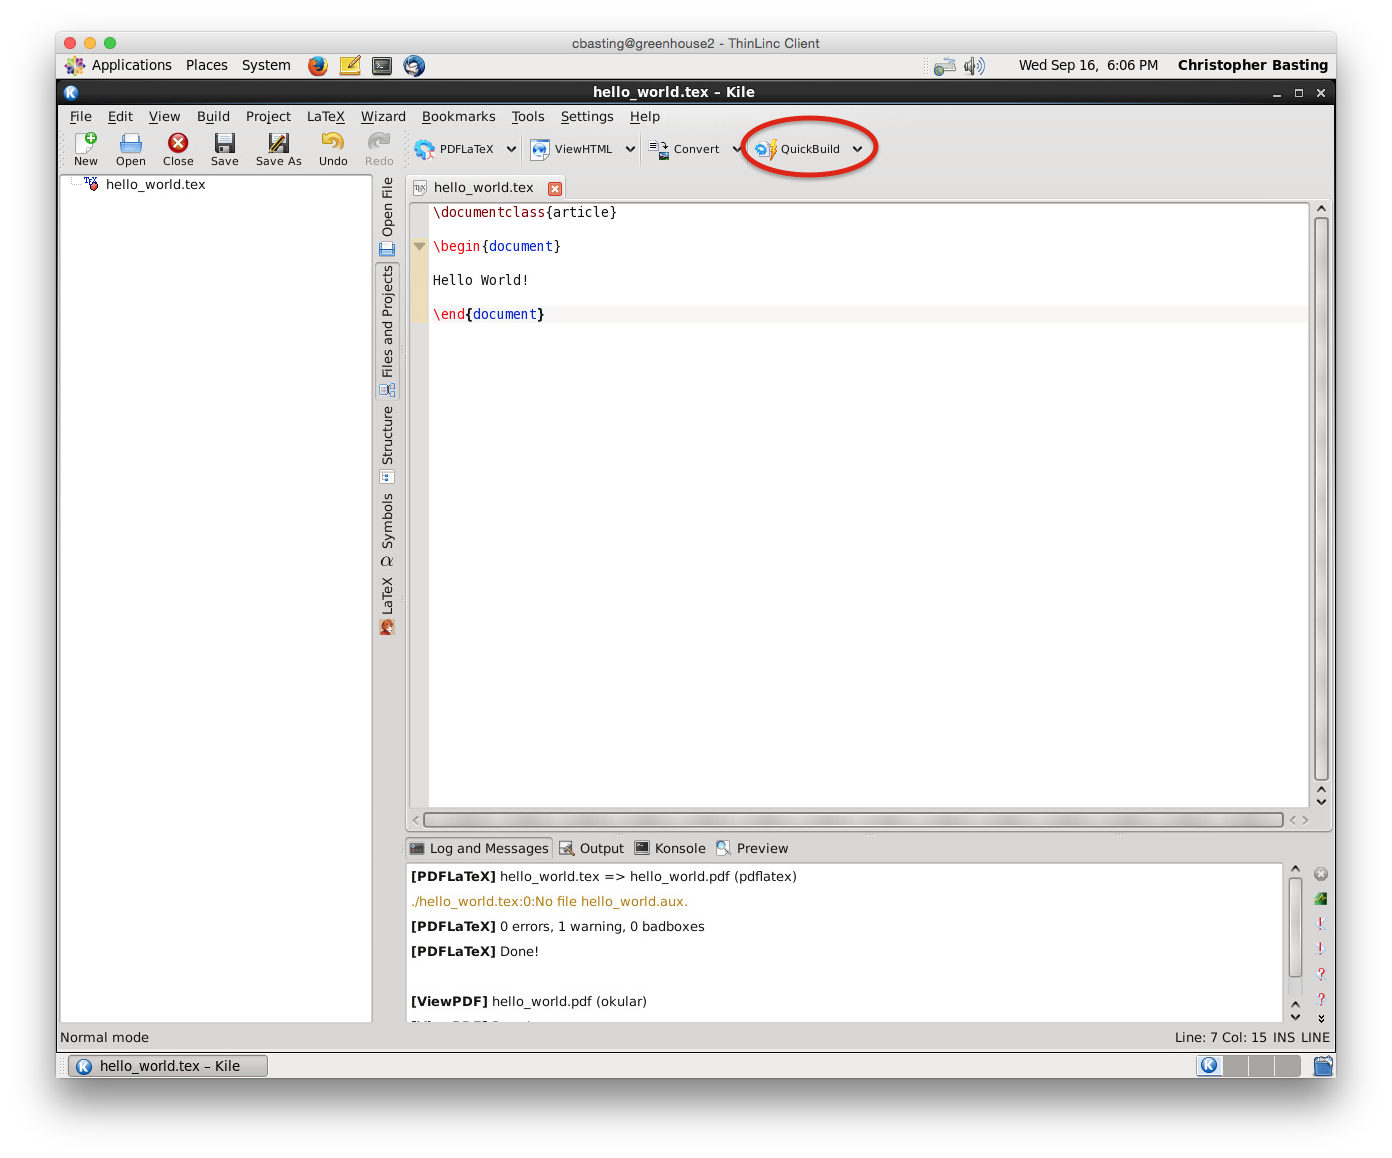
\includegraphics[width=\textwidth]{screenshots/kile-quickbuild.png}
\end{frame}

\begin{frame}[plain,noframenumbering]
	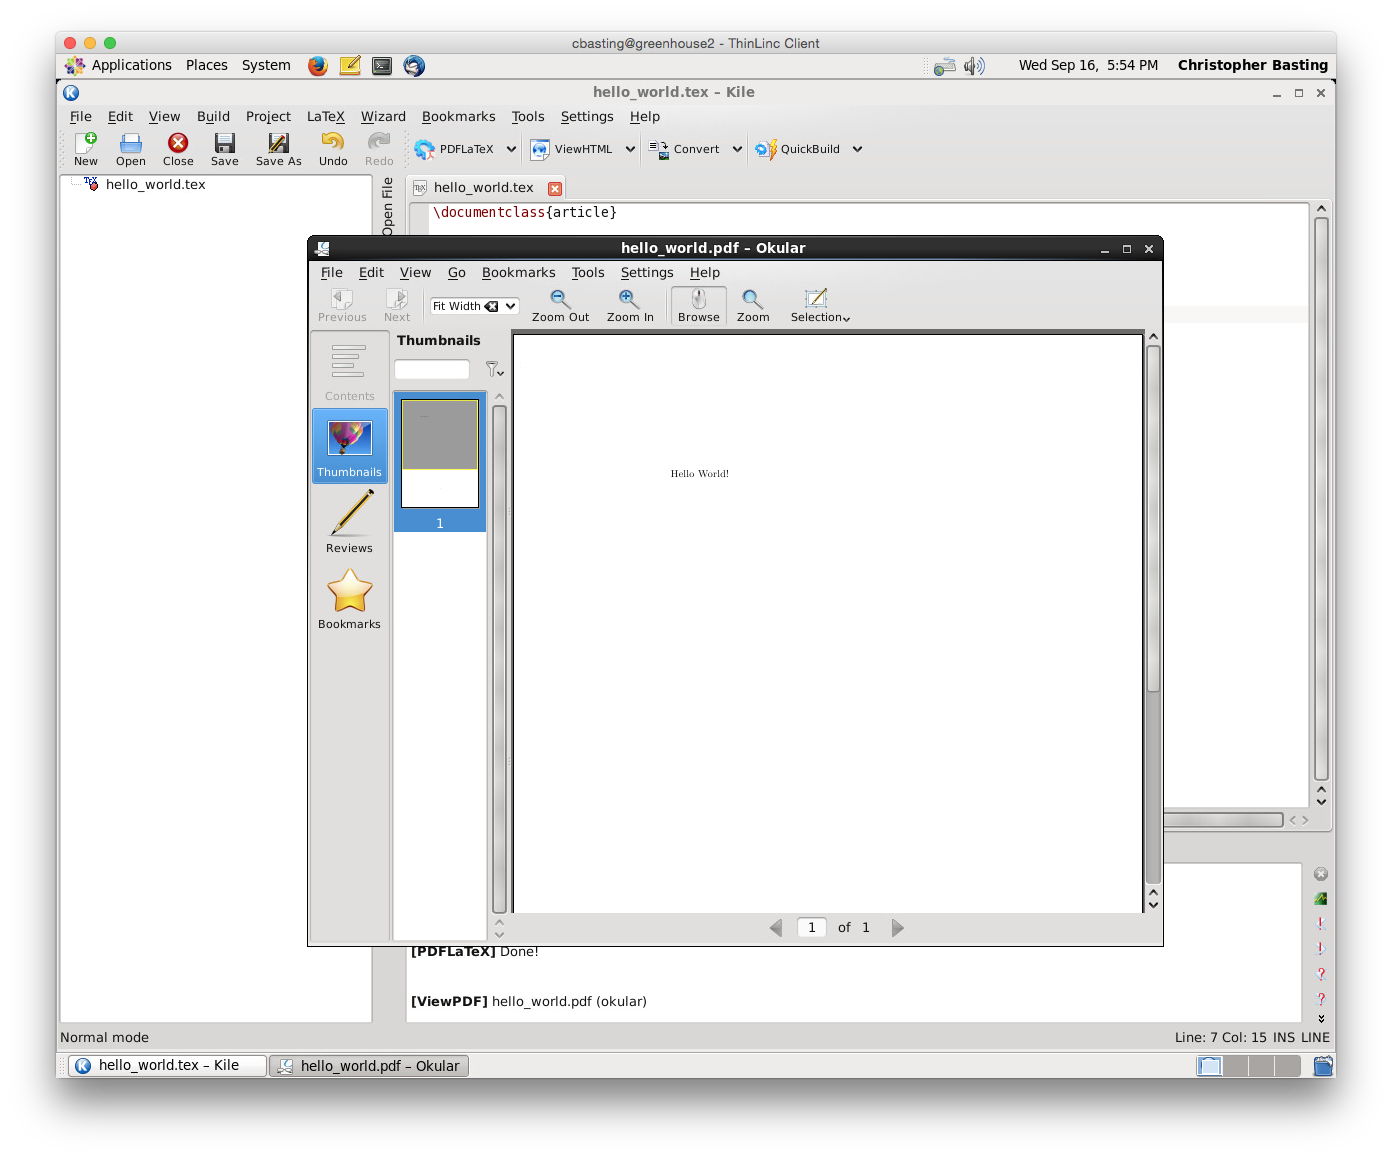
\includegraphics[width=\textwidth]{screenshots/kile-quickbuild-2.png}
\end{frame}

\begin{frame}[fragile]
	\frametitle{Hello World!}
	
	\latexBeispielDatei{Ein erstes \LaTeX-Dokument}{examples/hello_world/hello_world}
\end{frame}

\begin{frame}[fragile]
	\frametitle{Generierung einer PDF-Datei}
    Um eine PDF-Datei aus einem \LaTeX{} Dokument \dateiname{datei.tex} zu erzeugen, muss der \LaTeX-Compiler aufgerufen werden:\\
	\kommandozeile{pdflatex datei.tex} \\[1cm]
Alternativ kann man wie folgt vorgehen:
	\begin{enumerate}
		\item \kommandozeile{latex datei.tex}\\
		Dieser Befehl ruft den \LaTeX-Compiler auf und erzeugt die DVI-Datei \dateiname{datei.dvi}.
		\item \kommandozeile{dvips datei.dvi}\\
		Konvertiert die \dateiname{datei.dvi} in eine Post-Script Datei \dateiname{datei.ps}.
		\item \kommandozeile{ps2pdf} oder direkt \kommandozeile{dvipdf}\\
		Erzeugt eine PDF-Datei \dateiname{datei.pdf}.
	\end{enumerate}
\end{frame}

\begin{frame}
	\frametitle{Eingabe eines einfachen Textes}
	
	\latexBeispielDateiKlein{Quelltext}{examples/Eingabe_Quelltext/Eingabe_Quelltext}
\end{frame}

\begin{frame}
	\frametitle{Befehle und Umgebungen}
	\begin{itemize}
        \item \emphword{Befehle} haben in \LaTeX{} die Form \befehl{befehl}
		\item Beispiel: \befehl{textit\{kursiv\}} schaltet auf {\it Kursivschrift} um
		\item Manche Befehle benötigen zusätzliche Parameter, z. B.\\
		\befehl{textbf\{Text, der fett gedruckt sein soll\}}\\
		oder optionale Parameter, z. B.\\
		\befehl{documentclass[a4paper]\{article\}}\\[1cm]
		\item \emphword{Umgebungen} beeinflussen den gesamten enthaltenen Text:\\
		\befehl{begin\{center\}} \\
		~~~~zentrierter Text\\
		\befehl{end\{center\}}\\
		Auch hier ist die Angabe von Parametern möglich.
	\end{itemize}
\end{frame}
